\section{Penentuan Lokasi Sumber Suara}
\label{sec:sound_local}

Manusia dengan indra pendengaran yang berfungsi dengan baik dapat memperkirakan lokasi sumber suara. Ketika seseorang dipanggil oleh rekannya dari belakang, orang tersebut dapat memperkirakan bahwa suara panggilan berasal dari belakang sehingga orang tersebut akan menengok ke arah belakang. Selain itu, seseorang juga dapat memperkirakan arah (sudut) datangnya suara dengan indra pendengaran, yang lokasi sumber suaranya kemudian dapat dikonfirmasi oleh indra penglihatan setelah orang tersebut menengok ke arah perkiraan datangnya suara. Kemampuan menentukan lokasi sumber suara (\textit{sound localization}) yang dimiliki secara alami oleh manusia ini juga akan diimplementasikan pada agen virtual yang dihasilkan oleh RESTU.


\subsection{Penentuan Lokasi Sumber Suara Pada Manusia}
\label{subsec:human_sound_local}

Menurut para peneliti bidang psikoakustik, manusia menggunakan tiga dimensi dalam menentukan lokasi sumber suara \cite{goldstein2010}. Dimensi-dimensi tersebut adalah: (1) \textit{azimuth}, (2) elevasi, dan (3) jarak (\autoref{fig:psychoacoustic-dim}). Untuk menentukan \textit{azimuth}, manusia menggunakan parameter-parameter binaural, yaitu: (1) \textit{interaural time difference} (ITD); (2) \textit{interaural level difference} (ILD), yang dikenal juga sebagai \textit{interaural intensity difference} (IID); dan (3) perubahan spektral (\textit{coloration}) dari bunyi yang mencapai telinga bagian dalam \cite{goldstein2010, gelfand2010, kollmeier2008}. Untuk menentukan elevasi, manusia menggunakan parameter monaural berupa \textit{head-related transfer function} (HRTF). Sedangkan, untuk menentukan jarak, belum ada parameter yang pasti \cite{goldstein2010, gelfand2010}. Pada \autoref{sec:sound_local} ini, pembahasan terkait metode penentuan lokasi sumber suara pada manusia hanya mencakup parameter-parameter binaural, yaitu ITD dan ILD.

\begin{figure}[ht!]
\vskip 1em
\centering
 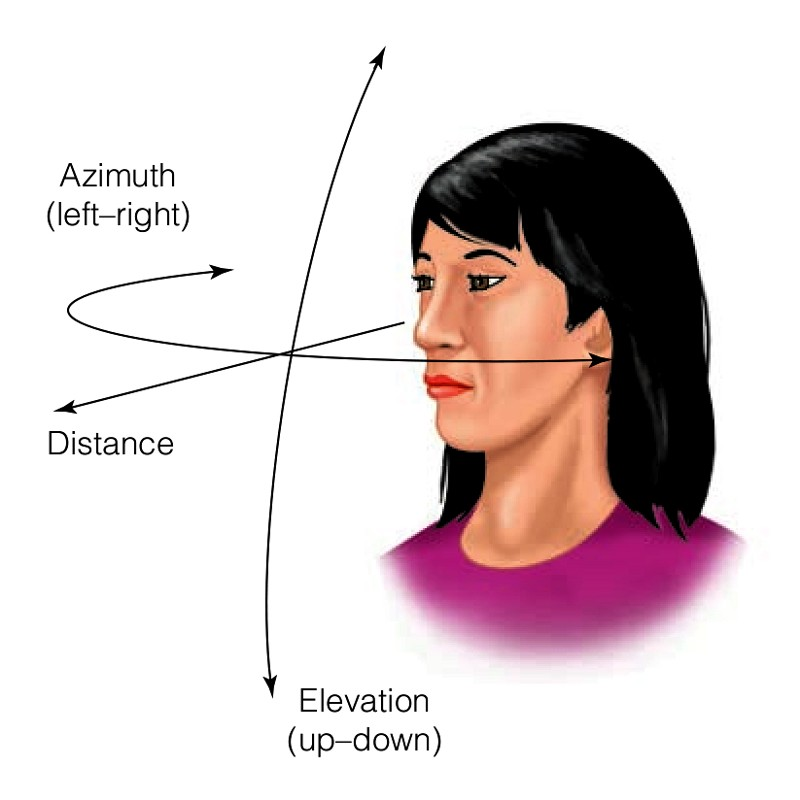
\includegraphics[width=.6\textwidth,keepaspectratio=true]{images/psychoacoustic-dim.jpg}
 \caption[Tiga dimensi yang digunakan manusia untuk menentukan lokasi sumber suara]{Tiga dimensi yang digunakan manusia untuk menentukan lokasi sumber suara \cite{goldstein2010}.}
 \label{fig:psychoacoustic-dim}
\vskip .5em
\end{figure} 

Parameter-parameter binaural didapatkan dengan membandingkan gelombang bunyi yang ditangkap oleh telinga kanan dan kiri. Pada ITD, variabel yang dibandingkan adalah waktu kedatangan gelombang bunyi pada kedua telinga tersebut. Apabila jarak sumber bunyi terhadap kedua telinga sama, misalnya sumber bunyi berada tepat di depan atau di belakang kepala pendengar, parameter ITD bernilai nol (titik A pada \autoref{fig:ilutrasi-itd}). Parameter ITD akan bernilai tidak nol apabila sumber bunyi berada pada \textit{azimuth} tertentu relatif terhadap arah depan kepala. Sebagai contoh, gelombang bunyi yang bersumber pada titik B (\autoref{fig:ilutrasi-itd}) akan diterima oleh telinga kanan terlebih dahulu. Pada gelombang sinusoidal, ITD akan bersifat ambigu antara \textit{leading} atau \textit{lagging} saat perbedaan fasa antara dua gelombang sinyal mencapai $180^o$. Oleh karena itu, ITD rentan menghasilkan nilai yang tidak tepat pada gelombang dengan frekuensi tinggi. 

Pada ILD atau IID, variabel yang dibandingkan adalah \textit{sound pressure level} (SPL) yang diterima oleh telinga kanan dan kiri. Perbedaan SPL yang diterima oleh kedua telinga disebabkan karena kepala membentuk sebuah \textit{acoustic shadow} yang meredam gelombang bunyi yang melaluinya, sehingga intensitas gelombang bunyi yang diterima oleh telinga yang jauh lebih kecil. Meskipun demikian, peredaman ini hanya signifikan pada gelombang dengan frekuensi tinggi (\autoref{fig:ilutrasi-ild-h} dan \autoref{fig:ilutrasi-ild-l}). Oleh karena itu, penentuan \textit{azimuth} lokasi sumber suara pada manusia mengombinasikan ITD dan ILD. ITD untuk gelombang bunyi dengan frekuensi rendah dan ILD untuk gelombang bunyi dengan frekuensi tinggi.

\begin{figure}[ht!]
\vskip 1em
\centering
 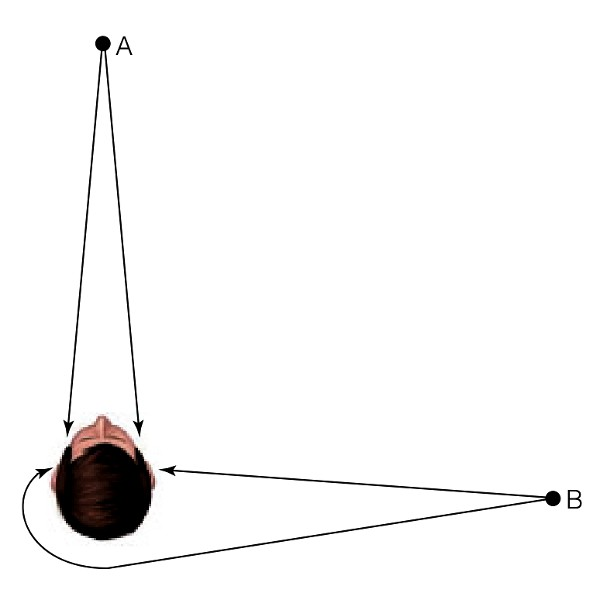
\includegraphics[width=.6\textwidth,keepaspectratio=true]{images/ilustrasi_itd.jpg}
 \caption[Ilustrasi \textit{interaural time difference} (ITD)]{Ilustrasi \textit{interaural time difference} (ITD) \cite{goldstein2010}.}
 \label{fig:ilutrasi-itd}
\vskip .5em
\end{figure}

\begin{figure}[ht!]
\vskip 1em
\centering
 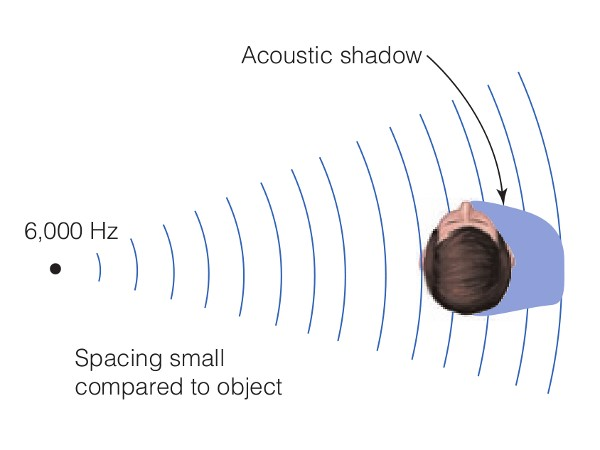
\includegraphics[width=.6\textwidth,keepaspectratio=true]{images/ilustrasi_ild_h.jpg}
 \caption[Ilustrasi \textit{interaural level difference} (ILD) pada gelombang dengan frekuensi tinggi]{Ilustrasi \textit{interaural level difference} (ILD) pada gelombang dengan frekuensi tinggi \cite{goldstein2010}.}
 \label{fig:ilutrasi-ild-h}
\vskip .5em
\end{figure}

\begin{figure}[ht!]
\vskip 1em
\centering
 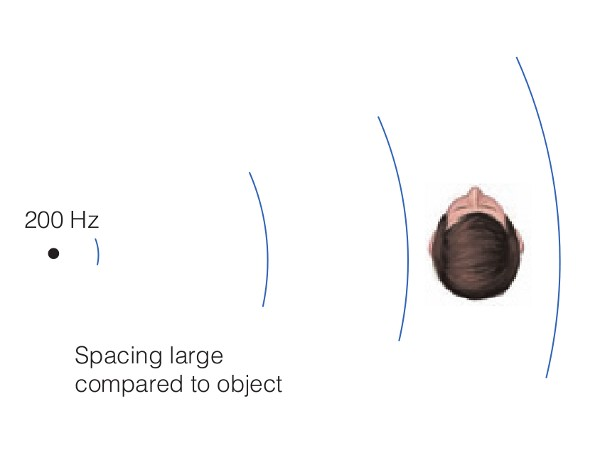
\includegraphics[width=.6\textwidth,keepaspectratio=true]{images/ilustrasi_ild_l.jpg}
 \caption[Ilustrasi \textit{interaural level difference} (ILD) pada gelombang dengan frekuensi rendah]{Ilustrasi \textit{interaural level difference} (ILD) pada gelombang dengan frekuensi rendah \cite{goldstein2010}.}
 \label{fig:ilutrasi-ild-l}
\vskip .5em
\end{figure}

Penentuan lokasi sumber suara yang digunakan RESTU untuk agen virtual (ECA) akan menggunakan konsep yang sama dengan ITD dan ILD, yaitu membandingkan waktu kedatangan dan amplitudo dari gelombang suara ucapan yang tertangkap oleh sepasang mikrofon.


\subsection{\textit{Time Difference of Arrival} (TDOA)}
\label{subsec:tdoa}

Parameter \textit{time difference of arrival} (TDOA) digunakan untuk mengukur perbedaan waktu kedatangan antara suara yang ditangkap oleh mikrofon yang satu dengan mikrofon yang lain dalam sebuah konfigurasi \textit{microphone array}. Pengukuran TDOA dikenal juga sebagai \textit{time delay estimation} (TDE), meskipun sebenarnya TDE sendiri dapat dibagi menjadi pengukuran TDOA dan pengukuran \textit{time of arrival} (TOA) \cite{huang2008}. Pada \autoref{sec:sound_local} ini, pembahasan metode TDE terbatas mengacu pada asumsi-asumsi yang telah didefinisikan pada \autoref{sec:batasan}.

Secara umum, dalam metode TDE terdapat dua model sinyal, yaitu model \textit{free-field} ideal dan model \textit{reverberant} \cite{huang2008, benesty2008}. Dalam \cite{chen2004}, terdapat satu model lagi yang disebut model \textit{multipath}. Tidak seperti model \textit{free-field} ideal yang hanya memperhitungkan sinyal yang bersifat \textit{direct path}, model \textit{multipath} dan model \textit{reverberant} memperhitungkan efek akustik dari ruangan, misalnya pantulan gelombang bunyi (\autoref{fig:propagation_model}). Perbedaan di antara keduanya adalah pada model \textit{multipath} jumlah pantulan dapat diperkirakan, sehingga jumlah \textit{path} gelombang dari sumber bunyi ke mikrofon dapat diketahui dan dapat dihitung. Pada model ini, terdapat variabel $\tau_{lm}$ yang menyatakan waktu tunda relatif antara mikrofon ke-$l$ dengan mikrofon ke-$0$ untuk \textit{path} ke-$m$, dengan $\tau_{01} = 0$. Sedangkan, pada model \textit{reverberant} jumlah \textit{path} sangat banyak sehingga nilai $\tau_{lm}$ sangat sulit untuk dihitung.


\begin{figure}[ht!]
\vskip 1em
\centering
 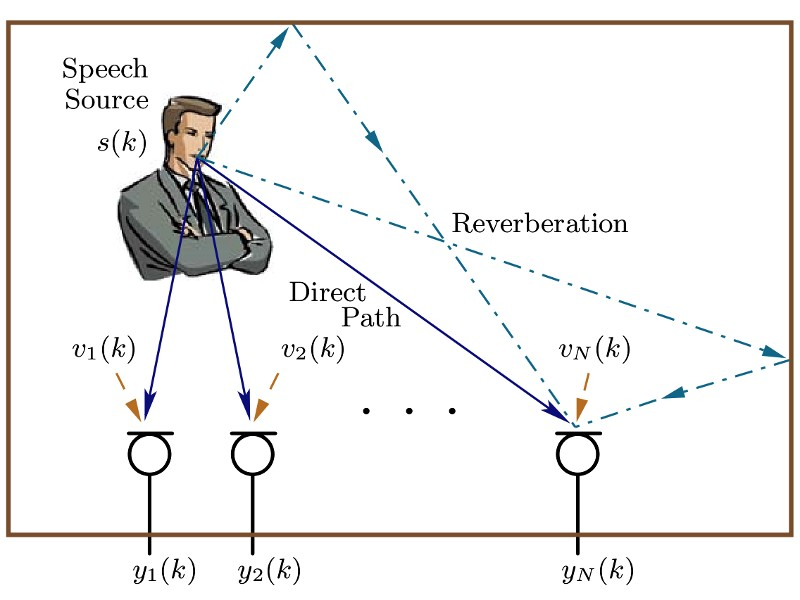
\includegraphics[width=.8\textwidth,keepaspectratio=true]{images/propagation_model.jpg}
 \caption[Ilustrasi model propagasi ideal dan model \textit{reverberant}]{Ilustrasi model propagasi ideal dan model \textit{reverberant} \cite{benesty2008}.}
 \label{fig:propagation_model}
\vskip .5em
\end{figure}


Model \textit{free-field} ideal, juga disebut sebagai model propagasi ideal, mengasumsikan bahwa mikrofon hanya menangkap sinyal yang bersifat \textit{direct path}. Dengan demikian, mikrofon diasumsikan menangkap sinyal yang teredam dan tertunda karena pengaruh propagasi dari sinyal asli yang dihasilkan oleh sumber suara, serta menangkap derau yang bersifat aditif. Mengacu ke skenario yang tergambar pada \autoref{fig:propagation_model}, sinyal yang ditangkap mikrofon $n$ dari sinyal $s$ pada waktu ke-$k$ dapat dinyatakan sebagai \autoref{eq:sinyal_ditangkap}.

\begin{equation}\label{eq:sinyal_ditangkap}
y_{n}(k) = \alpha_{n}s(k - \tau_{n}) + v_{n}(k), \qquad n = 1, 2, \cdots, N
\end{equation}

Pada \autoref{eq:sinyal_ditangkap} tersebut, $\alpha_{n}$ adalah faktor redaman karena propagasi ($0 \leq \alpha_{n} \leq 1$), $\tau_{n}$ adalah waktu yang dibutuhkan untuk propagasi, dan $v_{n}$ adalah derau aditif. Sinyal derau $v_{n}$ diasumsikan tidak berkorelasi dengan sinyal dari sumber suara dan derau yang tertangkap oleh mikrofon yang lain.

TDOA antara mikrofon ke-$i$ dan ke-$j$ dapat didefinisikan sebagai \autoref{eq:tdoa_mic_i_j}.

\begin{equation}\label{eq:tdoa_mic_i_j}
\tau_{ij} \triangleq \tau_{i} - \tau_{j}, \qquad i,j = 1, 2, \cdots, N
\end{equation}

Metode yang paling sederhana dan paling umum digunakan dalam menghitung TDOA adalah \textit{classical cross-correlation} (CCC) \cite{huang2008, benesty2008, chen2004}. Mengacu ke skenario yang tergambar pada \autoref{fig:propagation_model}, CCC antara sinyal $y_{1}(k)$ dan $y_{2}(k)$ dapat didefinisikan sebagai \autoref{eq:CCC_y1k_y2k}.

\begin{equation}\label{eq:CCC_y1k_y2k}
r^{CCC}_{y_{1} y_{2}} (p) = E [y_{1} (k) y_{2} (k + p)]
\end{equation}
 
Kemudian, TDOA dapat diperoleh dari \autoref{eq:tdoa_ccc}.

\begin{equation}\label{eq:tdoa_ccc}
\widehat{\tau}^{CCC}_{y_{1} y_{2}} = \operatorname*{arg\,max}_p r^{CCC}_{y_{1} y_{2}} (p)
\end{equation}

Pada \autoref{eq:CCC_y1k_y2k} dan \autoref{eq:tdoa_ccc}, $p \in [ -\tau_{max} , \tau_{max} ]$ dan $\tau_{max}$ adalah TDOA maksimum yang mungkin terjadi.

CCC sendiri merupakan kasus khusus dari \textit{generalized cross-correlation} (GCC) \cite{huang2008, benesty2008, chen2004}. TDOA pada GCC diperoleh dari \autoref{eq:tdoa_gcc}.

\begin{equation}\label{eq:tdoa_gcc}
\widehat{\tau}^{GCC}_{y_{1} y_{2}} = \operatorname*{arg\,max}_\tau r^{GCC}_{y_{1} y_{2}} (\tau)
\end{equation}

Sedangkan, persamaan GCC didefinisikan sebagai \autoref{eq:gcc_eq}.

\begin{align}\label{eq:gcc_eq}
r^{GCC}_{y_{1} y_{2}} (p) &= F^{-1} [ \Psi_{y_{1} y_{2}} (f) ] \nonumber \\
& = \int_{-\infty}^\infty \Psi_{y_{1} y_{2}} (f) e^{j 2 \pi f p} df \nonumber \\
& = \int_{-\infty}^\infty \vartheta (f) \phi_{y_{1} y_{2}} (f) e^{j 2 \pi f p} df
\end{align}

Pada \autoref{eq:gcc_eq} tersebut, $F^{-1} [ \cdot ]$ menyatakan \textit{inverse discrete-time Fourier transform} (IDTFT), $\Psi_{y_{1} y_{2}} (f)$ adalah \textit{generalized cross-spectrum}, dan $\phi_{y_{1} y_{2}} (f)$ adalah \textit{cross-spectrum}.

\textit{Cross-spectrum} didefinisikan sebagai \autoref{eq:cross_spectrum}, dengan $Y_n (f)$ didefinisikan sebagai \autoref{eq:transform_eq}.

\begin{equation}\label{eq:cross_spectrum}
\phi_{y_{1} y_{2}} (f) = E [ Y_1 (f) Y^*_2 (f) ]
\end{equation}

\begin{equation}\label{eq:transform_eq}
Y_n (f) = \sum_k y_n (k) e^{-j 2 \pi f k}, \qquad n = 1, 2
\end{equation}

Pada \autoref{eq:transform_eq}, $( \cdot )^*$ menyatakan konjugat kompleks.

\textit{Generalized cross-spectrum} didefinisikan sebagai \autoref{eq:gen_cross_spectrum}.

\begin{equation}\label{eq:gen_cross_spectrum}
\Psi_{y_{1} y_{2}} (f) = \vartheta (f) \phi_{y_{1} y_{2}} (f)
\end{equation}

Pada \autoref{eq:gen_cross_spectrum} tersebut, $\vartheta (f)$ adalah fungsi pembobotan pada domain frekuensi. Pada CCC, $\vartheta (f) = 1$.

Persamaan-persamaan GCC di atas dan hubungannya dengan CCC menunjukkan bahwa perhitungan CCC dapat dilakukan menggunakan \textit{discrete Fourier transform} (DFT) dan \textit{inverse} DFT (IDFT), yang dapat diimplementasikan secara efisien memanfaatkan \textit{fast Fourier transform} (FFT).


\subsection{\textit{Peak-to-Peak Amplitude Ratio} (PtPAR)}
\label{subsec:amplitude_ratio}

Parameter \textit{peak-to-peak amplitude ratio} (PtPAR) digunakan untuk mengukur perbedaan amplitudo gelombang antara sinyal suara yang ditangkap oleh mikrofon yang satu dengan mikrofon yang lain.

Intensitas gelombang suara pada sebuah ruang dapat dirumuskan sebagai \autoref{eq:intensitas_suara}.

\begin{equation}\label{eq:intensitas_suara}
I = \frac{P_{av}}{A} = \frac{P_{av}}{4 \pi r^2}
\end{equation}

Pada \autoref{eq:intensitas_suara} tersebut, $P_{av}$ adalah daya rata-rata yang dihasilkan oleh sumber suara, $A$ adalah luas permukaan bola, dan $r$ adalah jari-jari bola \cite{halliday2004}. Dengan demikian, hubungan antara intensitas gelombang suara $I$  dengan sebuah titik yang berjarak $r$ dari sumber suara dapat dinyatakan sebagai \autoref{eq:intensitas_jarak}.

\begin{equation} \label{eq:intensitas_jarak}
I \propto \frac{1}{r^2}
\end{equation}

Sedangkan, daya suatu gelombang dapat dirumuskan sebagai \autoref{eq:daya_gelombang}.

\begin{equation}\label{eq:daya_gelombang}
P = \frac{1}{2}	\mu \omega^2 A^2 v
\end{equation}

Pada \autoref{eq:daya_gelombang} tersebut, $\mu$ adalah rapat massa per satuan panjang medium, $\omega$ adalah frekuensi angular gelombang, $A$ adalah amplitudo gelombang, dan $v$ adalah cepat rambat gelombang \cite{halliday2004}. Dengan demikian, hubungan antara intensitas gelombang suara $I$ dengan amplitudo gelombang suara $A$ dapat dinyatakan sebagai \autoref{eq:intensitas_amplitudo}.

\begin{equation} \label{eq:intensitas_amplitudo}
I \propto {A^2}
\end{equation}

Dari \autoref{eq:intensitas_jarak} dan \autoref{eq:intensitas_amplitudo}, hubungan antara amplitudo gelombang suara $A$ dengan sebuah titik yang berjarak $r$ dari sumber suara dapat dinyatakan sebagai \autoref{eq:amplitudo_jarak}.

\begin{equation} \label{eq:amplitudo_jarak}
A \propto \frac{1}{r}
\end{equation}

Dengan demikian, hubungan perbandingan jarak titik 1 dan 2 dari sumber suara ($r_1$ dan $r_2$) dengan perbandingan amplitudo gelombang yang tertangkap pada kedua titik tersebut ($A_1$ dan $A_2$) dapat dinyatakan sebagai \autoref{eq:amplitudo_jarak_1}.

\begin{equation} \label{eq:amplitudo_jarak_1}
\frac{A_1}{A_2} = \frac{r_2}{r_1}
\end{equation}

Mengacu pada \autoref{eq:amplitudo_jarak} dan skenario yang tergambar pada \autoref{fig:propagation_model}, sinyal yang ditangkap mikrofon $n$ dari sinyal $s$ pada waktu ke-$k$ dengan mengabaikan waktu yang dibutuhkan oleh propagasi gelombang dapat dinyatakan dalam persamaan matematika sebagai \autoref{eq:sinyal_tanpa_propagasi}.

\begin{equation} \label{eq:sinyal_tanpa_propagasi}
y_{n}(k) = \frac{s(k)}{r_n} + v_{n}(k), \qquad n = 1, 2, \cdots, N
\end{equation}

Pada \autoref{eq:sinyal_tanpa_propagasi} tersebut, $r_{n}$ adalah jarak antara mikrofon $n$ dari sumber suara dan $v_{n}$ adalah derau aditif \cite{birchfield2005}.

Berdasarkan eksperimen yang dilakukan dalam \cite{birchfield2005}, dengan menggunakan parameter ILD saja, penentuan lokasi sumber suara dapat dilakukan secara akurat.